\clearpage % clear the prior chapter's page

\chapter{Evaluation of scoring approaches for integrative modeling using DEER distance data} \label{app:scoring}
%\vspace{-7mm}
%\bigskip

This Appendix is based on unpublished data.

%\vspace{-7mm}
\bigskip

Conformational changes define the functional cycles of many proteins. The complete characterization of functional intermediates, such as those that are infrequently sampled or are transiently populated, continues to elude established structural biology techniques. Integrating experimental distance data collected using \gls{deer} spectroscopy with computational modeling methods promises to overcome these barriers and provide a glimpse at these states. However, experimental \gls{deer} distance distributions cannot be reliably predicted or reproduced \emph{in silico}, preventing the identification of correctly folded models to high accuracy. In part because of this fact, the scoring functions used to evaluate protein structural models using experimental DEER data in the literature vary wildly and are highly non-standard. Here we use experimental data collected in the model system PfMATE to evaluate a panel of scoring functions with the goal of determining the most effective metric for identifying correctly folded protein structures. In general, most metrics were comparable in performance when scoring unimodal distributions consistent with a single structure. However, when the data indicated a bimodal distribution representing two populations in equilibrium, only a small subset of these metrics could effectively identify native-like models. We conclude that methods comparing the overlap between the simulated and experimental distributions, rather than their average distances as is commonly performed, are more effective at identifying native-like models when structural uniformity cannot be guaranteed by the data. Nevertheless, our results indicate that optimal results can only be achieved by \emph{a priori} determination of individual conformations in the data.

\section{Introduction}

The integration of sparse experimental data collected using \gls{cryoem}, X-ray crystallography, or \gls{nmr} with Rosetta protein structure prediction allows protein models to be generated at atomic-detail accuracy \citep*{Aprahamian2019, Boura2011, Srivastava2020, Steven2008, Xia2017}. Recently, distance data collected using \gls{epr} spectroscopy in conjunction with \gls{sdsl} have been a new focus for analyzing protein structure and dynamics \citep*{Hubbell2000, Hubbell2013, Jeschke2018a, Mchaourab2011}. Even a small number of distance measurements obtained using \gls{deer} spectroscopy, which range from \SIrange{15}{80}{\angstrom}, effectively complement short-range distance data obtained using nuclear magnetic resonance spectroscopy \citep*{Ling2016, Yang2010}. As a consequence, the number of computational tools that integrate these data into modeling continues to grow \citep*{Hays2019, Hirst2011, Marinelli2019}.

The recent interest in the \gls{deer} technique has been accompanied by methodological improvements in the way the primary spectroscopic data are converted in the distance restraints for computation. A number of paradigms exist for fitting these data \citep*{Srivastava2017, Worswick2018} with model-free fitting continuing to be the most widely-used strategy \citep*{Jeschke2006, Jeschke2002}. Recent studies have identified improvements in background correction methods \citep*{FabregasIbanez2020} and have detailed the optimal balance between fitting the data and regularization \citep*{Edwards2018, FabregasIbanez2019}. By contrast, among methods that model distributions as sums of Gaussian functions, substantial work has gone into identifying more effective fitting algorithms and model selection criteria \citep*{FabregasIbanez2020a, Hustedt2018, K.IlkerSen2007, Stein2015, Sweger2020}. In both cases, these advancements have coincided with the more widespread use of confidence bands in distance distributions to visualize experimental uncertainty \citep*{Edwards2016, FabregasIbanez2020a, Hustedt2018, Sweger2020}.

Less research has been completed into determining the best approach for converting these distance data into accurate protein structural models. As a result, there is no standard approach for integrating these data for protein structural modeling. For example, it is still common to use the average or peak distance as a single restraint while disregarding the width or shape of the distance distribution \citep*{Dastvan2016, Lim2018, VanEps2018}. In other cases, distribution widths have been used as function bounds \citep*{Alexander2008, Dastvan2016a, Evans2020, Fischer2016, Ling2016}. When spin labels are explicitly modeled as flexible side chains or pseudo-rotamers, restraints have been introduced that attempt to maximize the overlap between the entire simulated and experimental distributions \citep*{Hays2019, Kazmier2014a, Marinelli2015, Raghuraman2014, Roux2013}. A functionally similar approach is to minimize the area between the integrals \citep*{Krug2016}. Finally, the primary \gls{deer} data has been used directly for model-building and refinement \citep*{Bowen2018, Hilger2007, Marinelli2019, Reichel2018}. Although direct fitting has the potential to sidestep analytical artifacts, it is unclear whether there is any quantifiable improvement in model quality as a result of using this approach. Therefore, despite the variation in these approaches, to the best of our knowledge, the optimal scoring function for protein modeling has not been determined.

Here we employ the modeling suite Rosetta to compare several different scoring approaches using the proton-coupled multidrug transporter PfMATE as a model system. Different scoring functions are found to vary substantially in their ability to identify native-like structural models using sparse \gls{deer} data. Importantly, several commonly used metrics, such as naive integration of average distance values, fail to identify native-like models when the data are multimodal, which is commonly observed in conformationally heterogeneous proteins. Using scoring functions that compute the overlap between the experimental and simulated distributions could facilitate more meaningful interpretation of protein structures from limited \gls{deer} distance data.

\section{Results and Discussion}

\subsection{Overview of the hybrid energy function}

Protein structural models are commonly evaluated using a hybrid score representing the sum of its energy and its agreement with the data. This can be written as $E_{\mathup{total}}=E_{\mathup{model}} + w_{\mathup{data}} E_{\mathup{data}}$, where $E_{\mathup{model}}$ is a model’s score derived from an energy or scoring function, $E_{\mathup{data}}$ is the function evaluating a model’s goodness-of-fit to the experimental data, and $w_{\mathup{data}}$ is the weight assigned to the experimental data relative to the native energy function \citep*{Adams1997, Jack1978}. Ideally, both $E_{\mathup{model}}$ and $E_{\mathup{data}}$ would increase monotonically as a function of a model’s deviation from the target conformation of interest. In practice, neither term alone is sufficient to unequivocally identify the experimentally determined structure of a protein. The former crudely approximates the physical forces acting upon biomacromolecules in solution, while the latter reflects agreement with measurements that may be sparse, ambiguous, and unevenly distributed. Both functions must contribute to the calculation of physiologically meaningful models.

The challenge when applying experimental \gls{deer} data as modeling constraints is the fact that the distance distributions simulated \emph{in silico} tend to overstate the dynamics of the spin label while neglecting the dynamics of the protein backbone \citep*{Hagelueken2012, Hatmal2012, Islam2013, Polyhach2011}. Any single structural model can by definition only depict a subset of the backbone conformations sampled in solution. By contrast, because clash evaluation is predominantly used to remove rotamers from structural models, the conformations of the spin labels sampled in solution are likely a subset of the rotamer libraries used to simulate these distributions. As such, it is highly unlikely that any individual structural model can exactly reproduce the experimental data.

\subsection{Overview of the benchmark}

We thus sought to determine the most effective function of $E_{\mathup{data}}$ that could most effectively identify native-like models despite these factors. Several reasons guided the choice to use the multidrug transporter PfMATE as a model system to quantify the effectiveness of various scoring methods (Table \ref{tab:scoring_metrics}). First, several crystal structures in different conformations have previously been published \citep*{Tanaka2013, Zakrzewska2019}. Second, a comprehensive panel of experimental \gls{deer} data has been previously collected and found to be largely consistent with two of these structures that face either outward (to the periplasm) or inward (to the cytoplasm) \citep*{Jagessar2020}. Third, the Rosetta suite is well equipped to model intermediate states between these two conformations. We thus generated a library of "decoy" structural models of PfMATE using Rosetta by perturbing the dihedral angles of this helix, leading to approximately 3000 alternative conformations that ranged from \gls{of} to \gls{if}, fully occluded, and fully open (see Chapter \ref{ch:multilateration} for details on how these were modeled). We then calculated the $\mathrm{C_{\upalpha}}$ \gls{rmsd} of each model to the \gls{of} state. Finally, since this conformation is sampled at neutral pH, we curated four sets of distance distributions collected at pH 7.5 that interrogated this inter-lobe distance on both the intracellular and extracellular sides of the membrane (see Table \ref{tab:pfmate_restraints} in Chapter \ref{ch:multilateration}). 



\begin{table}[b!]
\scriptsize
\renewcommand{\tabcolsep}{0.15cm}
\centering
\caption[Scoring metrics used for the benchmark.]{Scoring metrics used for the benchmark. Symbols: $\mu$: average distance; $\sigma$: standard deviation; \emph{cdf}: cumulative density function; $p_{\mathit{X}} \left( r \right)$: probability of distance $r$ in distribution $X$.}

\newcolumntype{Y}{>{\raggedright\arraybackslash}X}

\begin{center}
\begin{tabular}{l c}
\toprule \\
\textbf{Method} & \textbf{Formula} \\
\midrule \\
Average distance only & $\left( \mu_{\mathup{sim}} - \mu_{\mathup{exp}} \right)^2$ \\
Bounded range & $ max \left( 0.0, | \mu_{\mathup{sim}} - \mu_{\mathup{exp}} - \sigma | \right) $ \\
Overlap & $ \sum_{\mathup{i}=1} | p_{\mathup{sim}} \left( r_{\mathup{i}} \right) - p_{\mathup{exp}} \left( r_{\mathup{i}} \right) | $  \\
Wasserstein & $\sum_{\mathup{i}=1} |cdf_{\mathup{sim}} \left( r_{\mathup{i}} \right) - cdf_{\mathup{exp}} \left( r_{\mathup{i}} \right) | $ \\
Discrepancy & $max \left( | p_{\mathup{sim}} \left( r \right) - p_{\mathup{exp}} \left( r \right) \right) $\\
Kolmogorov-Smirnov & $max \left( | cdf_{\mathup{sim}} \left( r \right) - cdf_{\mathup{exp}} \left( r \right) \right)$ \\
Chi-squared & $\sum_{\mathup{i}=1} \frac{ \left( p_{\mathup{sim}} \left( r_{\mathup{i}} \right) \right) - p_{\mathup{exp}} \left( r_{\mathup{i}} \right)^2 }{p_{\mathup{exp}} \left( r_{\mathup{i}} \right)} $ \\
Reverse Chi-squared & $\sum_{\mathup{i}=1} \frac{ \left( p_{\mathup{exp}} \left( r_{\mathup{i}} \right) \right) - p_{\mathup{sim}} \left( r_{\mathup{i}} \right)^2 }{p_{\mathup{sim}} \left( r_{\mathup{i}} \right)} $ \\
Cross entropy & $ - \sum_{\mathup{i}=1} p_{\mathup{exp}} \left( r_{\mathup{i}} \right) \ln \left( p_{\mathup{sim}} \left( r_{\mathup{i}} \right) \right) $ \\
Jensen-Shannon distance & $ \sqrt{ \sum_{\mathup{i}=1} \left( \frac{ p_{\mathup{sim}} \left( r_{\mathup{i}} \right) } {2} \ln \left( \frac{ 2 * p_{\mathup{sim}} \left( r_{\mathup{i}} \right) } {p_{\mathup{sim}} \left( r_{\mathup{i}} \right) + p_{\mathup{exp}} \left( r_{\mathup{i}} \right)} \right) \right) + \frac{ p_{\mathup{exp}} \left( r_{\mathup{i}} \right) } {2} \ln \left( \frac{ 2 * p_{\mathup{exp}} \left( r_{\mathup{i}} \right) } {p_{\mathup{sim}} \left( r_{\mathup{i}} \right) + p_{\mathup{exp}} \left( r_{\mathup{i}} \right)} \right) } $ \\
Bhattacharyya & $- \ln \left( \sum_{\mathup{i}=1} \sqrt{ p_{\mathup{sim}} \left( r_{\mathup{i}} \right) p_{\mathup{exp}} \left( r_{\mathup{i}} \right)}  \right)$ \\
Hellinger & $1 - \sum_{\mathup{i}=1} \sqrt{ p_{\mathup{sim}} \left( r_{\mathup{i}} \right) p_{\mathup{exp}} \left( r_{\mathup{i}} \right)} $\\
Jaccard index & $\sum_{\mathup{i}=1} \frac{ min \left( p_{\mathup{sim}} \left( r_{\mathup{i}} \right), p_{\mathup{exp}} \left( r_{\mathup{i}} \right) \right) } { max \left( p_{\mathup{sim}} \left( r_{\mathup{i}} \right), p_{\mathup{exp}} \left( r_{\mathup{i}} \right) \right)}$ \\
Joint probability & $\sum_{\mathup{i}=1} p_{\mathup{sim}} \left( r_{\mathup{i}} \right) p_{\mathup{exp}} \left( r_{\mathup{i}} \right)$ \\
\bottomrule \\
\end{tabular} 
\end{center}




\label{tab:scoring_metrics}
\end{table}

In addition to evaluating the effect of each function on scoring, we also focused on the contribution of experimental noise and uncertainty to scoring. The data preparation pipeline, which is discussed in detail in \ref{sec:scoring_methods}, proceeded as follows. First, the experimental distance data at pH 7.5 were converted into raw \gls{deer} traces in the time domain with a step size of \SI{8}{ns}. Background intermolecular coupling was modeled as a stretched exponential function with background slope values ranging from $10^{-6}$ to $10^{-1}$ and modulation depth values ranging uniformly from 0.05 to 0.40, which roughly corresponds to values that would be obtained with Q-band \gls{deer} without the use of an arbitrary waveform generator.  Second, random Gaussian noise was added to these time traces to simulate the effect of \gls{snr} that were either high (noise comprises 0.5\% of the signal on average), medium (2\%), or low (10\%). Third, these data were truncated at time window durations corresponding to the number of oscillations observed, which ranged from 0.2 to 3.0 with step sizes of 0.2. Previous research suggests that at least one complete oscillation is required to accurately resolve features in the distribution beyond the mean, such as the width and multimodality. Fourth, these data were converted into distance distributions with 95\% confidence intervals in an automated fashion using the analytical software DeerLab \citep*{FabregasIbanez2020a}. Finally, to evaluate the effect of restraint quantity on scoring, between one and ten such distributions were used as restraints to evaluate each structural model of PfMATE using each of the metrics listed in Table \ref{tab:scoring_metrics}.

\subsection{Unimodal distance distribution benchmark}

The results are presented in Figure \ref{fig:scoring_heatmap}.A and show that most metrics achieve Spearman correlation coefficients of approximately 0.7 under ideal conditions (three oscillations, ten restraints, high \gls{snr}). Interestingly, experimental \gls{snr}, but not duration in the time domain, appeared to have an outsized impact on correlation quality, which may be indicative of recent advancements in background correction methods during the analysis of \gls{deer} data \citep*{FabregasIbanez2020}. The least effective metrics for model quality by Spearman correlation were the average, cross-entropy, maximum discrepancy, and Chi-squared, each of which we discuss in turn. The average distance may have been overly sensitive to long-distance components that were occasionally added when time domain data were transformed to the distance domain, but which may be absent when more deliberate data analyses are performed. Indeed, simply using a distance range appeared to ameliorate this problem. The cross-entropy metric may have been sensitive to differences in the width of the experimental and simulated distributions, since it requires perfect overlap between the domains of the two distributions (e.g., the X-axes). This may be challenging for this specific model system, as the distance data are characterized by wide distributions likely resulting from backbone disorder. The discrepancy metric captures the largest difference in amplitudes at any point in the distance distribution; given the difficulty of exactly simulating \gls{deer} distance distributions \emph{in silico}, it is unsurprising that this a poor reporter for model quality. By contrast, we are unable to rationalize why the Chi-squared metric, but not the reverse Chi-squared metric, is ineffective of distinguishing native-like from non-native-like models. None of these results were substantially affected by the inclusion of 95\% confidence intervals during calculation (data not shown).

\begin{figure}[h!]
\centering
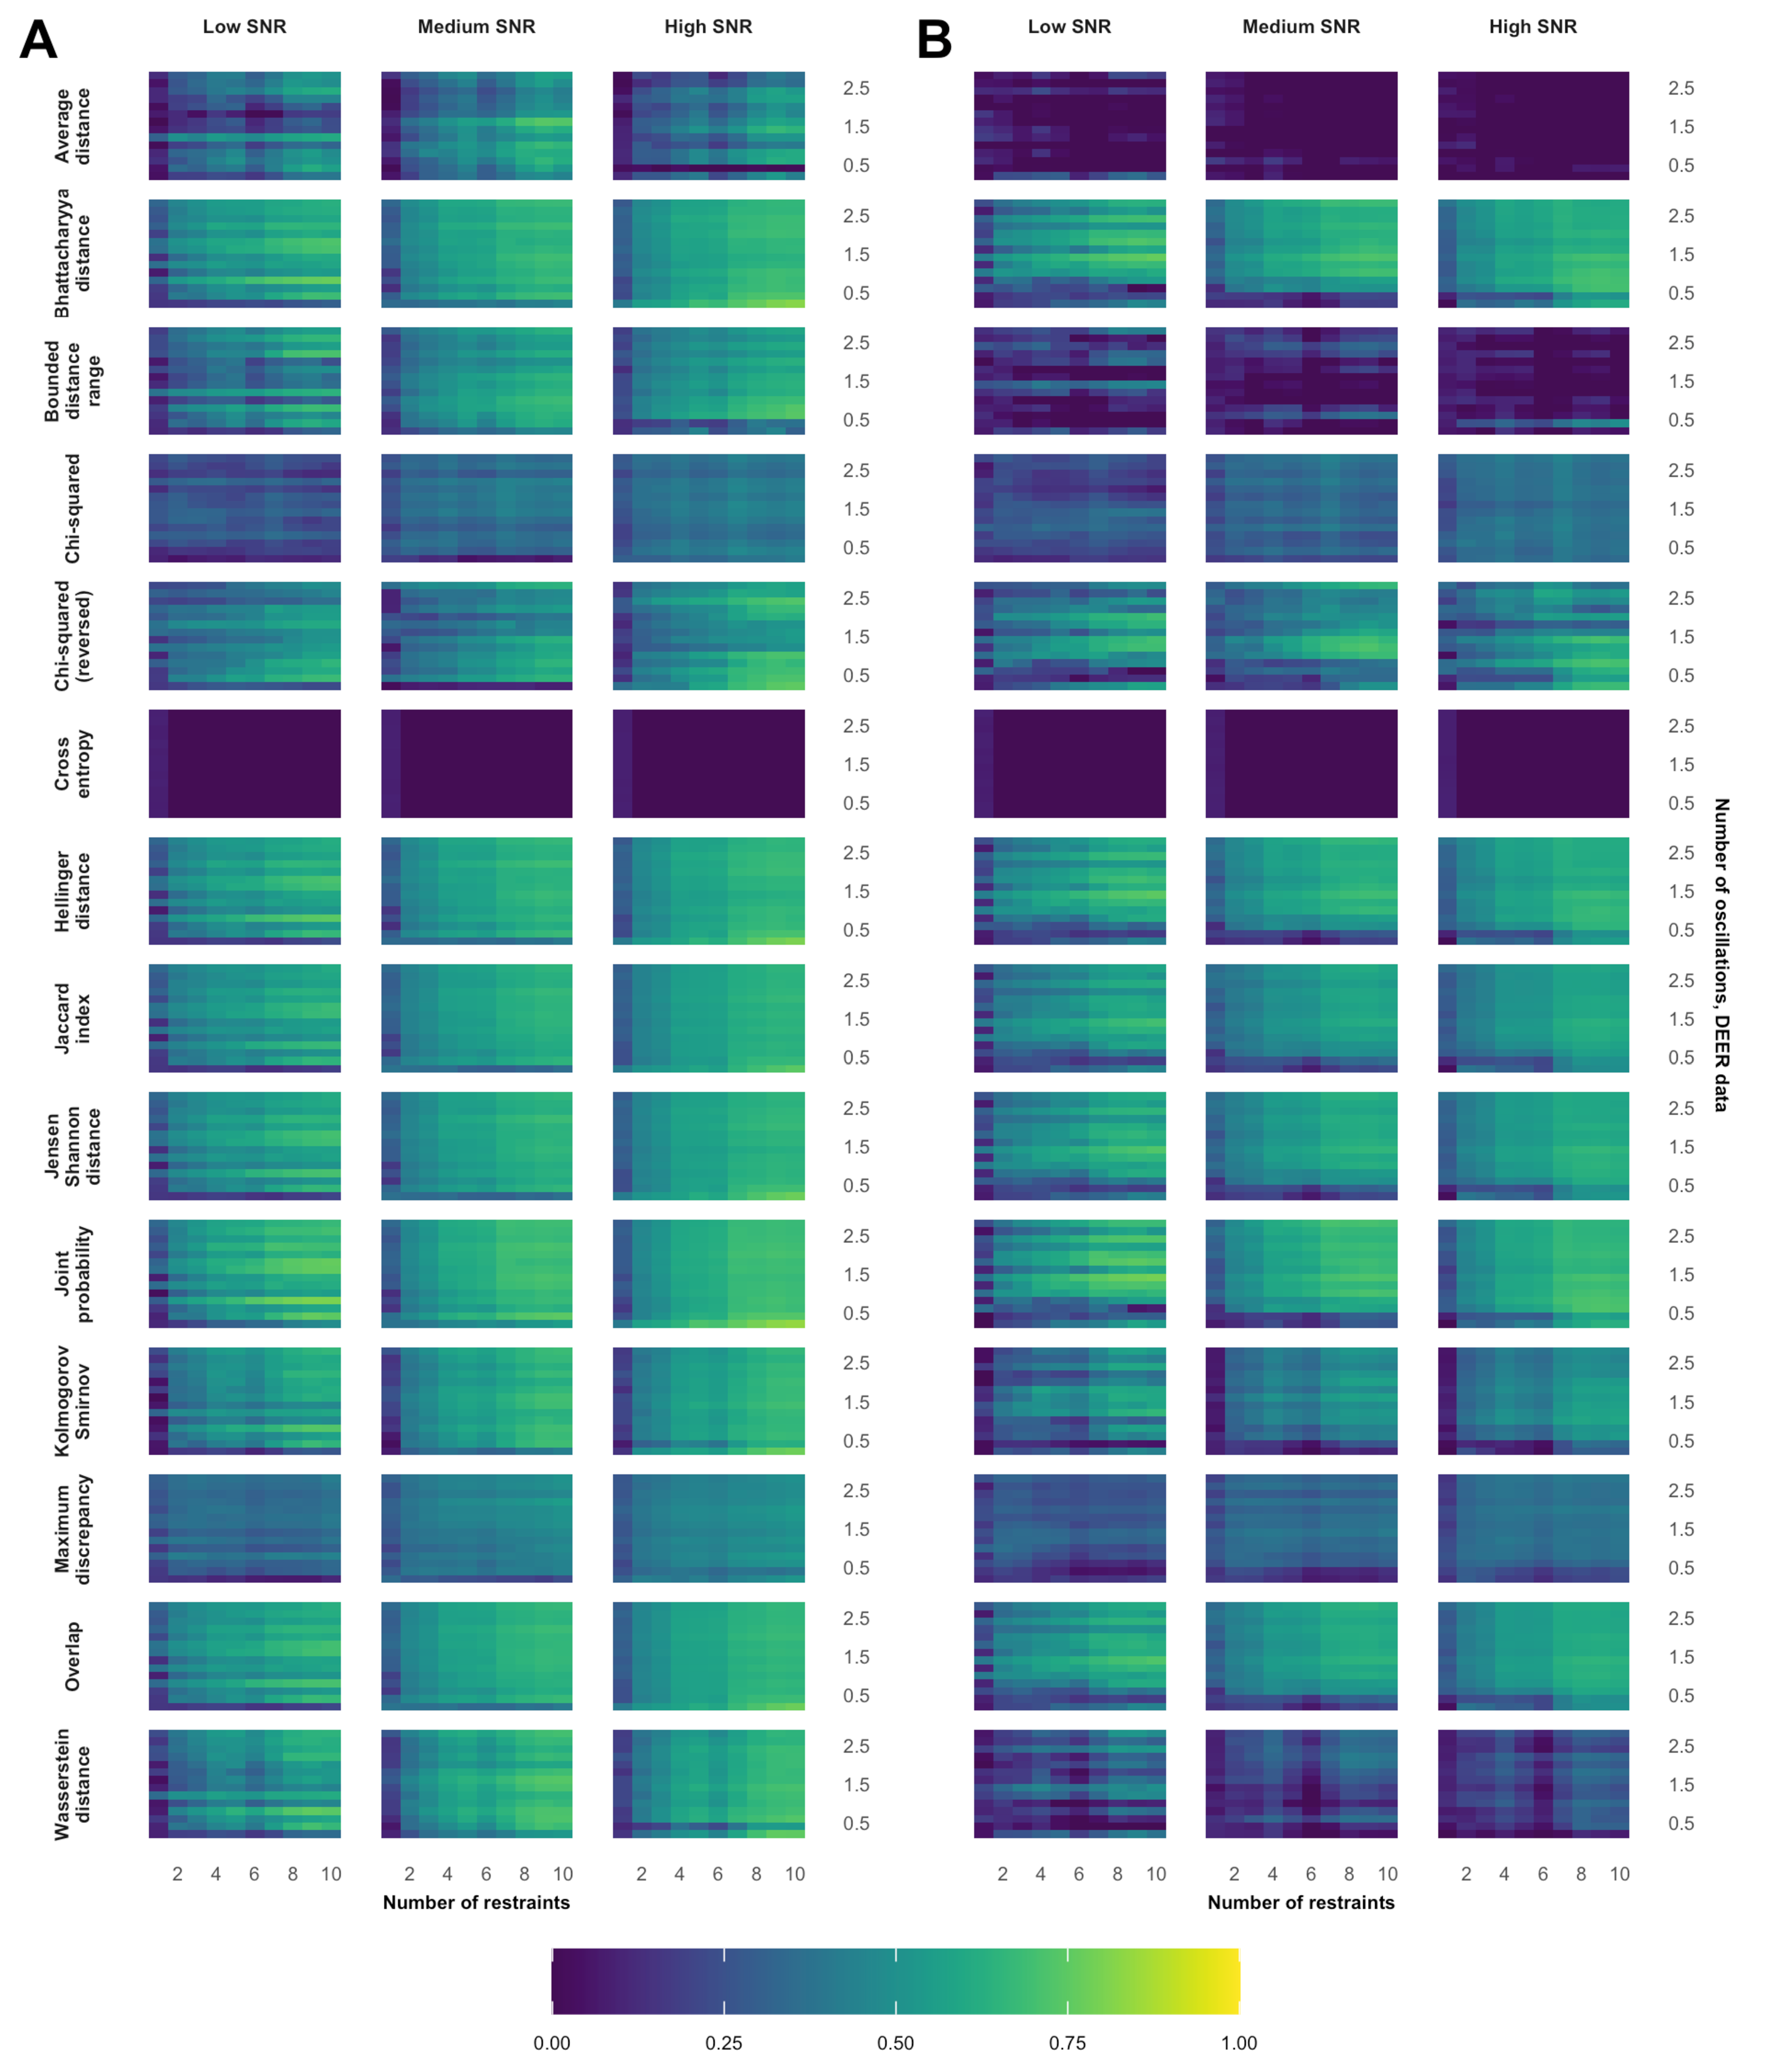
\includegraphics[width=6in]{Figures/scoring_heatmap.pdf}
 \caption[Spearman correlation coefficients between model RMSD and score as a function of number of restraints, number of oscillations in the data, and scoring function.]{Spearman correlation coefficients between model RMSD and score as a function of number of restraints, number of oscillations in the data, and scoring function. Data consist of distance distributions that are either A) unimodal or B) bimodal. Only a small number of metrics, namely those that evaluate the overlap between experimental and simulated \gls{deer} distance distributions, generate scores that correlate with \gls{rmsd} when using bimodal distributions.}
\label{fig:scoring_heatmap}
\end{figure}

\subsection{Multimodal distance distribution benchmark}

The results presented above are qualified by the fact that they were obtained using experimental data that is ideal for modeling purposes, insofar as they represent a single population or component consistent with the target crystal structure from which \gls{rmsd} values were measured. In practice, experimental data often features multiple populations with distinct distance components, some of which may be analytical artifacts or "ghost" peaks. While such data can be cleaned prior to modeling using strategies such as non-negative matrix factorization and/or global analysis \citep*{Hustedt2018, Wingler2019}, it is not always possible to exactly distinguish which distance components belong to the conformations of interest. Under circumstances where multiple components are present in the data, we would expect metrics that consider agreement with entire distributions, such as the average distance, or the Wasserstein (also called the earth mover's) distance quantifying the area between the integrals of two distributions, to be overly sensitive, and thus respond poorly, to multimodality in the data.

To test this hypothesis, we repeated the simulation pipeline outlined above, but added a distance component consistent with the \gls{if} conformation of PfMATE prior to simulation of the data in the time domain. The remaining steps of the analytical pipeline were unchanged. Each distribution in this second set of data thus consisted of an even mixture of distance components belonging to outward- and inward-facing PfMATE. The results, plotted in Figures \ref{fig:scoring_heatmap}.B and \ref{fig:scoring_comparison}, reveal that the majority of metrics considered in this study are incapable of correctly identifying models using these data, with many of their respective correlation coefficients plummeting even under ideal conditions (three oscillations, high \gls{snr}, ten restraints). Because performance was irrespective of \gls{snr} or duration in the time domain, we believe these reflect fundamental shortcomings in the ways scores are computed, rather than how the data were analyzed. We note that results obtained using these distributions, unlike the unimodal distributions discussed above, appeared to be more sensitive to time domain truncation, which may reflect the increased difficulty of resolving the shape of these distribution when there is insufficient data in the time domain.

\begin{figure}[h]
\centering
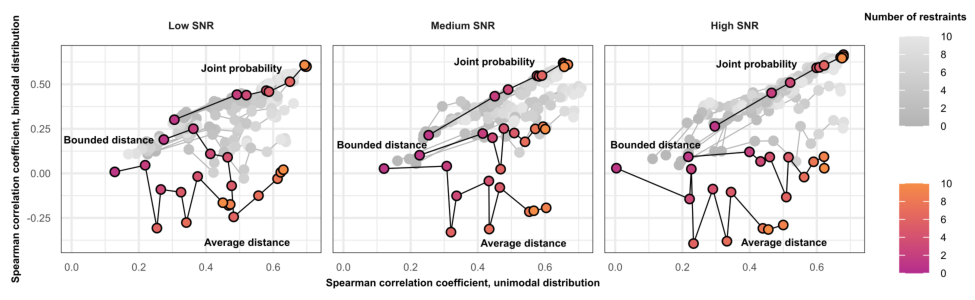
\includegraphics[width=6in]{Figures/scoring_comparison.pdf}
 \caption[Comparison of scoring methods when evaluating unimodal and bimodal distributions.]{Comparison of scoring methods when evaluating unimodal and bimodal distributions. All data used for scoring results shown here consisted of three oscillations in the time domain.}
\label{fig:scoring_comparison}
\end{figure}

Correlation coefficients calculated using several methods, such as the Jaccard index and the Joint probability, appear to be minimally affected by the presence of new components in the distance data. Interestingly, these metrics all favorably score partial overlap between distance components, while penalizing distributions that fall between the two components. This may allow specific conformations consistent with the data to be pinpointed, including the outward-open conformation from which RMSD values were calculated. It should be noted that these methods were more sensitive to time domain truncation than the unimodal distributions described above, which may demonstrate the extent to which low-quality data interferes with high-precision modeling of protein structures. Nonetheless, all of them return values that correlate slightly worse than when scoring models using unimodal distributions (Figure \ref{fig:scoring_heatmap}.A), again demonstrating the value of preprocessing the data prior to modeling.

\subsection{Concluding remarks}

This study evaluated several scoring functions using experimental \gls{deer} data in the conformationally heterogeneous model system PfMATE. We elected to use this model system, rather than a more static system such as T4 Lysozyme, due to its nonnegligible backbone dynamics that are also observed in other proteins of biophysical interest \citep*{Collauto2017, Dastvan2019, Evans2020, Martens2016, Verhalen2017a}. Indeed, while these experimental data may be broadly classified as consisting of components belonging to either outward-facing or inward-facing conformations, they also indicate substantial heterogeneity and disorder. Thus, reducing the distribution to a single value, such as an average distance, appears in this case to be detrimental to high-precision modeling. In general, the majority of scoring functions studied here return values that correlate well with model quality when the data consist of only one component. By contrast, while none of these scoring functions perfectly maintain this performance when the data consist of multiple components, a minority of these scoring functions can nonetheless return score values for models that correlate with \gls{rmsd}. Nevertheless, in all cases the Spearman correlation coefficients decreased, indicating the importance of preprocessing the data and, if possible, isolating individual components in the data prior to modeling.

\section{Materials and Methods}\label{sec:scoring_methods}

\subsection{Preparation of PfMATE decoy models}

A library of 2,855 structural models of PfMATE was generated using the software suite Rosetta 3.10 \citep*{Leaver-fay2011, Leman2020}, with both its \gls{of} (PDB: 6GWH) and \gls{if} (PDB: 6FHZ) conformations serving as template models. These models were generated using fragment insertion, in which the backbone dihedral angles of transmembrane helices 1 (residues 1-50) and 7 (residues 240-268) were perturbed using sequence fragments obtained from the Protein Databank. Sequence fragments were obtained from the Robetta web server as previously described \citep*{Kim2004}. A total of 5000 rounds of fragment insertion was executed using the scoring function \emph{score3}. Each model's structural similarity to the outward-facing state (PDB: 6GWH) was then calculated using the \emph{score\_jd2} application with residues 1-50 omitted. Finally, we binned these models by this \gls{rmsd} value and balanced the dataset to avoid the overrepresentation of models that were either fully occluded or highly inaccurate.

\subsection{Simulation and analysis of DEER data}

All experimental \gls{deer} distributions used in this study have been previously published \citep*{Jagessar2020}. Unimodal distance distributions were simulated using the data at pH 7.5 as follows. First, each distance distribution was converted into a \gls{deer} trace in the time domain with \SI{8}{ns} time steps as previously described. Each trace was normalized such that the signal intensity at \SI{0}{\upmu s} was equal to 1, and their duration was set to three oscillations, which we calculated from the average distance $r_{\mathup{avg}}$ in angstroms such that one oscillation had a duration of $ \frac{r_{\mathup{avg}}^3}{5.2*10^4} $ microseconds. Second, background coupling was simulated using the function $B \left(t \right)=\exp \left( -kt \right)$, where $k$ represents the contribution of intermolecular background coupling to the signal and $t$ is the time in microseconds. Then, normally distributed noise was added to simulate the contribution of experimental noise in the data, with the standard deviation equal to either 0.005, 0.02, or 0.1 for the high, medium, and low \gls{snr} datasets, respectively. Finally, these \gls{deer} traces were truncated to specific durations ranging from 0.2 to 3.0 oscillations and were analyzed using the \emph{fitmodel} function implemented in DeerLab v0.13.1 with default settings \citep*{FabregasIbanez2020a}.

Simulation of bimodal distributions was identical, except the experimental \gls{deer} data collected at pH 4.0 were added to the experimental distributions collected at pH 7.5 prior to transformation to the time domain.

\subsection{Scoring of PfMATE models using simulated DEER distributions}

We used the \emph{score\_jd2} application to score each PfMATE model using each of the metrics listed in Table \ref{tab:scoring_metrics}. All scoring methods were implemented in RosettaDEER. Scores were correlated with \gls{deer} values using the \emph{spearmanr} function as implemented in SciPy \citep*{Virtanen2020}.

\section{Acknowledgements}

We would like to thank Luis Fábregas Ibáñez for helpful assistance with DeerLab and Karan Bhardwaj for contributing exploratory data analysis to this study.